\documentclass{standalone}

\usepackage[english]{babel}
\usepackage[utf8x]{inputenc}
\usepackage[T1]{fontenc}
\usepackage{tikz,pgf} %and any other packages or tikzlibraries your picture needs
\usepackage{amsfonts}
\usepackage{amsmath}
\usepackage{physics}
\usepackage{amssymb}
\usepackage{mathtools}
\usetikzlibrary{shapes,arrows,patterns}

\begin{document}

%%%%%%%%%%%%%%%%%%%%%%%%%%%%%%%%%%%%%%%%%%%%%%%%%%%%%%%%%%%%%%%%%%%%%%%%%%%%%%%%
%COPY HERE
%%%%%%%%%%%%%%%%%%%%%%%%%%%%%%%%%%%%%%%%%%%%%%%%%%%%%%%%%%%%%%%%%%%%%%%%%%%%%%%%



\tikzset{every picture/.style={line width=0.75pt}} %set default line width to 0.75pt

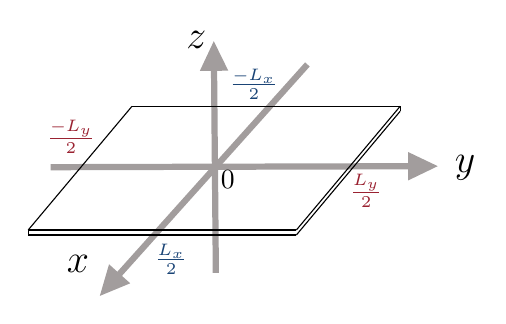
\begin{tikzpicture}[x=0.75pt,y=0.75pt,yscale=-1,xscale=1]
%uncomment if require: \path (0,300); %set diagram left start at 0, and has height of 300

%Straight Lines [id:da3003250640268105]
\draw [color={rgb, 255:red, 162; green, 157; blue, 157 }  ,draw opacity=1 ][line width=2.25]    (181.4,159.55) -- (362.9,159.06) ;
\draw [shift={(367.9,159.05)}, rotate = 539.85] [fill={rgb, 255:red, 162; green, 157; blue, 157 }  ,fill opacity=1 ][line width=0.08]  [draw opacity=0] (14.29,-6.86) -- (0,0) -- (14.29,6.86) -- cycle    ;
%Straight Lines [id:da8689546067621734]
\draw [color={rgb, 255:red, 162; green, 157; blue, 157 }  ,draw opacity=1 ][line width=2.25]    (305.1,110.05) -- (208.44,217.83) ;
\draw [shift={(205.1,221.55)}, rotate = 311.89] [fill={rgb, 255:red, 162; green, 157; blue, 157 }  ,fill opacity=1 ][line width=0.08]  [draw opacity=0] (14.29,-6.86) -- (0,0) -- (14.29,6.86) -- cycle    ;
%Straight Lines [id:da7970692632058651]
\draw [color={rgb, 255:red, 162; green, 157; blue, 157 }  ,draw opacity=1 ][line width=2.25]    (261,210.5) -- (260.04,103.83) ;
\draw [shift={(260,98.83)}, rotate = 449.49] [fill={rgb, 255:red, 162; green, 157; blue, 157 }  ,fill opacity=1 ][line width=0.08]  [draw opacity=0] (14.29,-6.86) -- (0,0) -- (14.29,6.86) -- cycle    ;
%Straight Lines [id:da3519471636626119]
\draw    (170.6,189.8) -- (299.8,189.8) ;
%Straight Lines [id:da7963832060808382]
\draw    (299.8,189.8) -- (349.8,130.2) ;
%Straight Lines [id:da6491507288076224]
\draw    (220.6,130.2) -- (349.8,130.2) ;
%Straight Lines [id:da39220315951527485]
\draw    (170.6,189.8) -- (220.6,130.2) ;
%Straight Lines [id:da03581404411817579]
\draw    (170.6,192.2) -- (299.8,192.2) ;
%Straight Lines [id:da6682783230769427]
\draw    (299.8,192.2) -- (349.8,132.6) ;
%Straight Lines [id:da3091548050753099]
\draw    (170.6,189.8) -- (170.6,192.2) ;
%Straight Lines [id:da8752360367747976]
\draw    (349.8,130.2) -- (349.8,132.6) ;

% Text Node
\draw (187.9,200.93) node [anchor=north west][inner sep=0.75pt]  [font=\Large]  {$x$};
% Text Node
\draw (374.9,152.6) node [anchor=north west][inner sep=0.75pt]  [font=\Large]  {$y$};
% Text Node
\draw (245.57,92.6) node [anchor=north west][inner sep=0.75pt]  [font=\Large]  {$z$};
% Text Node
\draw (230.24,195.27) node [anchor=north west][inner sep=0.75pt]  [font=\small,color={rgb, 255:red, 26; green, 68; blue, 118 }  ,opacity=1 ]  {$\frac{L_{x}}{2}$};
% Text Node
\draw (266.24,110.93) node [anchor=north west][inner sep=0.75pt]  [font=\small,color={rgb, 255:red, 26; green, 68; blue, 118 }  ,opacity=1 ]  {$\frac{-L_{x}}{2}$};
% Text Node
\draw (178.24,135.6) node [anchor=north west][inner sep=0.75pt]  [font=\small,color={rgb, 255:red, 154; green, 34; blue, 49 }  ,opacity=1 ]  {$\frac{-L_{y}}{2}$};
% Text Node
\draw (324.24,161.6) node [anchor=north west][inner sep=0.75pt]  [font=\small,color={rgb, 255:red, 154; green, 34; blue, 49 }  ,opacity=1 ]  {$\frac{L_{y}}{2}$};
% Text Node
\draw (262.17,159.73) node [anchor=north west][inner sep=0.75pt]  [font=\normalsize]  {$0$};


\end{tikzpicture}

%%%%%%%%%%%%%%%%%%%%%%%%%%%%%%%%%%%%%%%%%%%%%%%%%%%%%%%%%%%%%%%%%%%%%%%%%%%%%%%%
%COPY HERE
%%%%%%%%%%%%%%%%%%%%%%%%%%%%%%%%%%%%%%%%%%%%%%%%%%%%%%%%%%%%%%%%%%%%%%%%%%%%%%%%

\end{document}
